% ============================================================================
%  PLANTILLA LaTeX PARA APUNTES UNIVERSITARIOS
%  Materias: MPI I, Lógica Computacional, Programación C++
%  Universidad: UNAHUR (Universidad Nacional de Hurlingham)
%  Compilar con: pdflatex template-apunte.tex (2 pasadas)
% ============================================================================

% ────────────────────────────────────────────────────────────────────────────
%  PREÁMBULO: todo lo que va ANTES de \begin{document}
% ────────────────────────────────────────────────────────────────────────────

% documentclass: define el tipo de documento.
%   [11pt]     = tamaño de fuente principal
%   [a4paper]  = papel A4 (el estándar en Argentina)
%   {article}  = clase artículo (capítulos NO, secciones SÍ)
\documentclass[11pt,a4paper]{article}

%% ─── PAQUETES ESENCIALES ───────────────────────────────────────────────────

% Codificación de caracteres: permite usar tildes, ñ, etc. en el .tex
% UTF-8 es el estándar, asegurate de GUARDAR EL ARCHIVO COMO UTF-8.
\usepackage[utf8]{inputenc}

% Font encoding: para que el PDF muestre bien las tildes y caracteres
\usepackage[T1]{fontenc}

% Idioma español (argentino). Opciones útiles:
%   es-tabla   = cambia "Cuadro" por "Tabla" (más correcto en español)
%   es-nolists = no traduce los entornos de listas (itemize, enumerate)
\usepackage[spanish,es-tabla]{babel}

%% ─── PAQUETES DE MATEMÁTICAS ───────────────────────────────────────────────

% amsmath  = paquete principal para matemáticas (ecuaciones, align, cases, etc.)
% amssymb  = símbolos matemáticos extra (\mathbb, \therefore, \forall, etc.)
% amsthm   = entornos para teoremas, definiciones, demostraciones
\usepackage{amsmath,amssymb,amsthm}

%% ─── PAQUETES DE DISEÑO Y MAQUETACIÓN ─────────────────────────────────────

% geometry: controla los márgenes de la página.
%   margin=2.5cm  = los 4 márgenes a 2.5 cm. Se puede ajustar:
%   Ej: top=3cm, bottom=2cm, left=2.5cm, right=2.5cm
\usepackage[margin=2.5cm]{geometry}

% fancyhdr: encabezados y pies de página personalizados
\usepackage{fancyhdr}

% multicol: texto en varias columnas (útil para glosarios, resúmenes)
\usepackage{multicol}

% enumitem: control avanzado sobre listas (itemize, enumerate, description)
% Permite cambiar espaciado, numeración, etc.
\usepackage{enumitem}

%% ─── PAQUETES DE GRÁFICOS E IMÁGENES ──────────────────────────────────────

% graphicx: para incluir imágenes (jpg, png, pdf)
%   \includegraphics[width=...]{archivo}
\usepackage{graphicx}

% xcolor: colores para texto, tablas, código, TikZ, etc.
%   Se pueden definir colores personalizados con \definecolor
\usepackage{xcolor}

% tikz: paquete para hacer diagramas (Venn, árboles, autómatas, grafos)
% Requiere al menos una compilación extra a veces.
\usepackage{tikz}

%% ─── CÓDIGO FUENTE (listings) ──────────────────────────────────────────────

% listings: muestra código fuente formateado (C++, Python, etc.)
\usepackage{listings}

%% ─── TABLAS AVANZADAS ──────────────────────────────────────────────────────

% booktabs: produce líneas horizontales profesionales (\toprule, \midrule, \bottomrule)
\usepackage{booktabs}

% array: características extra para columnas en tablas
\usepackage{array}

%% ─── HIPERVÍNCULOS ─────────────────────────────────────────────────────────

% hyperref: convierte las referencias cruzadas en hipervínculos en el PDF.
% Debe cargarse AL FINAL del preámbulo (después de los otros paquetes).
\usepackage[
    colorlinks=true,       % los links se ven de color (no rectángulos)
    linkcolor=blue,        % color de links internos (índice, figuras)
    citecolor=green,       % color de citas bibliográficas
    urlcolor=blue,         % color de URLs
    breaklinks=true,       % permite que los links largos se corten entre líneas
    bookmarks=true,        % crea marcadores en el PDF
    bookmarksnumbered=true % los marcadores llevan números
]{hyperref}

% ────────────────────────────────────────────────────────────────────────────
%  CONFIGURACIÓN DE LISTINGS (CÓDIGO FUENTE)
% ────────────────────────────────────────────────────────────────────────────

%% DEFINICIÓN DE COLORES PERSONALIZADOS
% Formato: \definecolor{nombre}{modelo}{definición}
% Modelos comunes: rgb (0-1), HTML (00-ff), cmyk
\definecolor{codegreen}{rgb}{0,0.5,0}
\definecolor{codegray}{rgb}{0.5,0.5,0.5}
\definecolor{codepurple}{rgb}{0.58,0,0.82}
\definecolor{codeblue}{rgb}{0,0,0.7}
\definecolor{backcolour}{rgb}{0.95,0.95,0.92}
\definecolor{codecyan}{rgb}{0,0.5,0.5}

%% ESTILO PERSONALIZADO PARA CÓDIGO C++
% Se aplica con: \lstset{style=cppstyle}  o  \lstinputlisting[style=cppstyle]{archivo.cpp}
\lstdefinestyle{cppstyle}{
    language=C++,                 % lenguaje: C++
    backgroundcolor=\color{backcolour}, % color de fondo
    commentstyle=\color{codegreen},     % color de comentarios
    keywordstyle=\color{codeblue},      % color de palabras clave
    stringstyle=\color{codepurple},     % color de cadenas de texto
    numberstyle=\tiny\color{codegray},  % estilo de números de línea
    basicstyle=\ttfamily\small,         % fuente: monoespaciada, tamaño small
    breaklines=true,               % partir líneas largas automáticamente
    showstringspaces=false,        % no mostrar ▯ en espacios de cadenas
    numbers=left,                  % números de línea a la izquierda
    numbersep=5pt,                 % separación entre número y código
    frame=single,                  % recuadro alrededor del código
    tabsize=4,                     % tamaño de la tabulación
    captionpos=b,                  % posición del título: bottom (abajo)
    % escapeinside={\%*}{*)},     % (OPCIONAL) para escribir LaTeX dentro del código
    showtabs=false,                % no marcar tabulaciones
    showspaces=false               % no marcar espacios
}

% Aplicamos el estilo por defecto (así todos los lstlisting lo usan)
\lstset{style=cppstyle}

% ────────────────────────────────────────────────────────────────────────────
%  ENTORNOS DE TEOREMAS (amsthm)
% ────────────────────────────────────────────────────────────────────────────
% amsthm provee 3 estilos predefinidos:
%   \theoremstyle{definition} → texto normal, título en negrita
%   \theoremstyle{plain}      → texto en itálica, título en negrita
%   \theoremstyle{remark}     → texto normal, título en itálica
%
% Los entornos se numeran por sección con [section]:
%   Ej: "Definición 1.1", "Definición 1.2", etc.

\theoremstyle{definition}
\newtheorem{definicion}{Definición}[section]
\newtheorem{ejemplo}{Ejemplo}[section]
\newtheorem{ejercicio}{Ejercicio}[section]

\theoremstyle{plain}
\newtheorem{teorema}{Teorema}[section]
\newtheorem{lema}{Lema}[section]
\newtheorem{corolario}{Corolario}[section]

\theoremstyle{remark}
\newtheorem{observacion}{Observación}[section]
\newtheorem{nota}{Nota}[section]

% El entorno {proof} ya viene definido por amsthm.
% Se usa: \begin{proof}...\end{proof}
% Opcionalmente: \begin{proof}[Demostración alternativa]...\end{proof}

% ────────────────────────────────────────────────────────────────────────────
%  CONFIGURACIÓN DE ENCABEZADOS Y PIES (fancyhdr)
% ────────────────────────────────────────────────────────────────────────────

% Primero, activamos el estilo fancy
\pagestyle{fancy}

% Limpiamos encabezados y pies por defecto
\fancyhf{}

% Configuramos encabezado:
%   L = Left (izquierda), C = Center (centro), R = Right (derecha)
%   \leftmark  = nombre de la sección actual (mayúsculas por defecto)
%   \rightmark = nombre de la subsección actual
\fancyhead[L]{\leftmark}
\fancyhead[R]{\thepage}

% Pie de página (opcional, se puede dejar vacío)
\fancyfoot[C]{\small \textit{Apunte de estudio --- UNAHUR}}

% Línea horizontal en el encabezado (por defecto está activa)
\renewcommand{\headrulewidth}{0.4pt}

% Línea horizontal en el pie (0pt = invisible)
\renewcommand{\footrulewidth}{0pt}

% ────────────────────────────────────────────────────────────────────────────
%  OTROS AJUSTES
% ────────────────────────────────────────────────────────────────────────────

% Para que \leftmark muestre el nombre de sección como aparece (sin mayúsculas)
% \markboth{izquierda}{derecha} — el primer argumento es para \leftmark,
% el segundo para \rightmark.
\renewcommand{\sectionmark}[1]{\markboth{#1}{}}

% Espaciado entre párrafos (en vez de sangría)
% Descomentar si se prefiere:
% \setlength{\parskip}{1em}
% \setlength{\parindent}{0pt}

% ────────────────────────────────────────────────────────────────────────────
%  INICIO DEL DOCUMENTO
% ────────────────────────────────────────────────────────────────────────────
% Todo lo que escribas después de \begin{document} y antes de \end{document}
% aparecerá en el PDF.
% ────────────────────────────────────────────────────────────────────────────

\begin{document}

%% ===========================================================================
%%  PORTADA (TITLE PAGE)
%% ===========================================================================
% \maketitle genera la portada usando \title, \author, \date.
% Si querés una portada más elaborada, podés usar el entorno {titlepage}.

\title{%
    % Si tenés un logo institucional, lo podés incluir así:
    % \begin{center}
    %   \includegraphics[width=4cm]{logo-unahur.png}
    % \end{center}
    % \vspace{1cm}
    {\huge \textbf{Apunte de Lógica Proposicional}} \\[0.5cm]
    {\large MPI I --- Lógica Computacional} \\
    {\large Universidad Nacional de Hurlingham}
}

\author{%
    Alumno: Juan Pérez \\[0.3cm]
    {\small \textit{Cambiar estos datos por los propios}} \\
    {\small Este template es un punto de partida para crear apuntes}
}

% \date{15 de julio de 2026}   % Fecha fija
\date{\today}                   % Fecha automática (día de compilación)

% Generamos la portada
\maketitle

\thispagestyle{empty}  % La portada no lleva número de página
\newpage

%% ===========================================================================
%%  ÍNDICE (TABLE OF CONTENTS)
%% ===========================================================================
% \tableofcontents genera el índice automáticamente.
% Requiere COMPILAR DOS VECES: primero genera el .toc, segundo lo lee.
\tableofcontents
\newpage

%% ===========================================================================
%%  SECCIÓN 1: LÓGICA PROPOSICIONAL
%% ===========================================================================
% \section{...} crea una sección.
% Se numera automáticamente: 1, 2, 3...
% Para secciones sin número: \section*{...} (no aparecen en el índice)

\section{Introducción a la Lógica Proposicional}

% ────────────────────────────────────────────────────────────────────────────
%  SUBSECCIÓN 1.1: Definición de proposición
% ────────────────────────────────────────────────────────────────────────────

\subsection{¿Qué es una proposición?}

\begin{definicion}[Proposición]
Una \textbf{proposición} es una oración declarativa que puede ser verdadera (V)
o falsa (F), pero no ambas simultáneamente.
\end{definicion}

\begin{ejemplo}
Las siguientes son proposiciones:
\begin{itemize}
    \item \texttt{``2 + 2 = 4''}  (verdadera)
    \item \texttt{``El cielo es verde''}  (falsa)
    \item \texttt{``5 es un número primo''}  (verdadera)
\end{itemize}

No son proposiciones:
\begin{itemize}
    \item \texttt{``¿Qué hora es?''}  (pregunta, no declara)
    \item \texttt{``x + 1 = 5''}  (no es V ni F hasta que se defina x)
    \item \texttt{``¡Cállate!''}  (orden, no declaración)
\end{itemize}
\end{ejemplo}

% ────────────────────────────────────────────────────────────────────────────
%  SUBSECCIÓN 1.2: Conectivos lógicos
% ────────────────────────────────────────────────────────────────────────────

\subsection{Conectivos lógicos}

Las proposiciones pueden combinarse mediante \textbf{conectivos lógicos}
(también llamados \textit{operadores lógicos}) para formar proposiciones
más complejas.

\begin{definicion}[Conectivos básicos]
Los cinco conectivos fundamentales son:

\begin{center}
\begin{tabular}{lccc}
\toprule
\textbf{Nombre} & \textbf{Símbolo} & \textbf{Significado} & \textbf{Se lee} \\
\midrule
Negación    & $\lnot$ & $\lnot p$ & ``no p'' \\
Conjunción  & $\land$ & $p \land q$ & ``p y q'' \\
Disyunción  & $\lor$  & $p \lor q$  & ``p o q'' \\
Implicación & $\to$   & $p \to q$   & ``si p entonces q'' \\
Doble implicación & $\leftrightarrow$ & $p \leftrightarrow q$ & ``p si y solo si q'' \\
\bottomrule
\end{tabular}
\end{center}
\end{definicion}

% ────────────────────────────────────────────────────────────────────────────
%  SUBSECCIÓN 1.3: Tablas de verdad
% ────────────────────────────────────────────────────────────────────────────

\subsection{Tablas de verdad}

Una \textbf{tabla de verdad} muestra el valor de verdad de una proposición
compuesta para todas las combinaciones posibles de sus variables.

\begin{ejemplo}[Tabla de verdad de $p \land q$]
La conjunción es verdadera únicamente cuando \textbf{ambas} proposiciones
lo son:

\begin{center}
\begin{tabular}{c|c|c}
$p$ & $q$ & $p \land q$ \\
\midrule
V & V & \textbf{V} \\
V & F & F \\
F & V & F \\
F & F & F
\end{tabular}
\end{center}
\end{ejemplo}

\begin{ejemplo}[Tabla completa de conectivos]
Veamos todos los conectivos juntos:

\begin{center}
\begin{tabular}{c|c|c|c|c|c}
$p$ & $q$ & $\lnot p$ & $p \land q$ & $p \lor q$ & $p \to q$ \\
\midrule
V & V & F & V & V & V \\
V & F & F & F & V & F \\
F & V & V & F & V & V \\
F & F & V & F & F & V
\end{tabular}
\end{center}

Notar que la implicación $p \to q$ solo es falsa cuando el antecedente
($p$) es verdadero y el consecuente ($q$) es falso.
\end{ejemplo}

% ────────────────────────────────────────────────────────────────────────────
%  SUBSECCIÓN 1.4: Leyes de De Morgan
% ────────────────────────────────────────────────────────────────────────────

\subsection{Leyes de De Morgan}

Las \textbf{leyes de De Morgan} son dos equivalencias lógicas
fundamentales que relacionan la negación con la conjunción y la disyunción.

\begin{teorema}[Leyes de De Morgan]
Para cualesquiera proposiciones $p$ y $q$:
\begin{align}
    \lnot (p \land q) &\equiv \lnot p \lor \lnot q \label{eq:dm1} \\
    \lnot (p \lor q)  &\equiv \lnot p \land \lnot q \label{eq:dm2}
\end{align}
\end{teorema}

\begin{observacion}
En español coloquial, la primera ley se lee:
``La negación de (p y q) equivale a (no p) o (no q)''.
Intuitivamente: si no es cierto que ambas son verdaderas, entonces
al menos una es falsa.
\end{observacion}

% ────────────────────────────────────────────────────────────────────────────
%  SUBSECCIÓN 1.5: Demostración
% ────────────────────────────────────────────────────────────────────────────

\subsection{Ejemplo de demostración}

\begin{ejemplo}[Demostrar una equivalencia lógica]
Demostrar la siguiente equivalencia usando tablas de verdad:
\[
p \to q \equiv \lnot p \lor q
\]

\begin{proof}
Construimos la tabla de verdad para ambas expresiones:

\begin{center}
\begin{tabular}{c|c|c|c|c}
$p$ & $q$ & $\lnot p$ & $\lnot p \lor q$ & $p \to q$ \\
\midrule
V & V & F & V & V \\
V & F & F & F & F \\
F & V & V & V & V \\
F & F & V & V & V
\end{tabular}
\end{center}

Como las columnas de $\lnot p \lor q$ y $p \to q$ coinciden para
todas las combinaciones de $p$ y $q$, queda demostrada la equivalencia.
\end{proof}
\end{ejemplo}

%% ===========================================================================
%%  SECCIÓN 2: SÍMBOLOS MATEMÁTICOS ÚTILES
%% ===========================================================================
% Esta sección funciona como referencia rápida de símbolos.

\section{Símbolos matemáticos de MPI I}

\subsection{Lógica proposicional}

\begin{center}
\begin{tabular}{lll}
\toprule
\textbf{Comando} & \textbf{Símbolo} & \textbf{Significado} \\
\midrule
\texttt{\textbackslash{}land}  & $\land$ & conjunción (y) \\
\texttt{\textbackslash{}lor}   & $\lor$  & disyunción (o) \\
\texttt{\textbackslash{}lnot}  & $\lnot$ & negación (no) \\
\texttt{\textbackslash{}to}    & $\to$   & implicación \\
\texttt{\textbackslash{}leftrightarrow} & $\leftrightarrow$ & doble implicación \\
\texttt{\textbackslash{}equiv} & $\equiv$ & equivalencia lógica \\
\texttt{\textbackslash{}top}   & $\top$   & verdadero (tautología) \\
\texttt{\textbackslash{}bot}   & $\bot$   & falso (contradicción) \\
\texttt{\textbackslash{}Rightarrow}  & $\Rightarrow$ & implica (consecuencia) \\
\texttt{\textbackslash{}Leftrightarrow} & $\Leftrightarrow$ & si y solo si \\
\bottomrule
\end{tabular}
\end{center}

\subsection{Conjuntos}

\begin{center}
\begin{tabular}{lll}
\toprule
\textbf{Comando} & \textbf{Símbolo} & \textbf{Significado} \\
\midrule
\texttt{\textbackslash{}in}     & $\in$   & pertenece \\
\texttt{\textbackslash{}notin}  & $\notin$ & no pertenece \\
\texttt{\textbackslash{}subseteq} & $\subseteq$ & subconjunto \\
\texttt{\textbackslash{}subset} & $\subset$ & subconjunto propio \\
\texttt{\textbackslash{}cup}    & $\cup$  & unión \\
\texttt{\textbackslash{}cap}    & $\cap$  & intersección \\
\texttt{\textbackslash{}emptyset} & $\emptyset$ & conjunto vacío \\
\texttt{\textbackslash{}mathbb\{N\}} & $\mathbb{N}$ & naturales \\
\texttt{\textbackslash{}mathbb\{Z\}} & $\mathbb{Z}$ & enteros \\
\texttt{\textbackslash{}mathbb\{Q\}} & $\mathbb{Q}$ & racionales \\
\texttt{\textbackslash{}mathbb\{R\}} & $\mathbb{R}$ & reales \\
\bottomrule
\end{tabular}
\end{center}

\subsection{Cuantificadores}

\begin{center}
\begin{tabular}{lll}
\toprule
\textbf{Comando} & \textbf{Símbolo} & \textbf{Significado} \\
\midrule
\texttt{\textbackslash{}forall} & $\forall$ & para todo \\
\texttt{\textbackslash{}exists} & $\exists$ & existe \\
\texttt{\textbackslash{}nexists} & $\nexists$ & no existe \\
\texttt{\textbackslash{}exists!} & $\exists!$ & existe un único \\
\texttt{\textbackslash{}therefore} & $\therefore$ & por lo tanto \\
\texttt{\textbackslash{}because} & $\because$ & porque \\
\bottomrule
\end{tabular}
\end{center}

%% ===========================================================================
%%  SECCIÓN 3: MATEMÁTICAS AVANZADAS (ejemplos de uso)
%% ===========================================================================
% Esta sección muestra cómo usar distintos entornos matemáticos.
% Todos son de uso común en MPI I y Lógica Computacional.

\section{Ejemplos de entornos matemáticos}

\subsection{Ecuaciones inline y display}
\label{sec:inline-display}

Las ecuaciones \textbf{inline} van entre \texttt{\$...\$} y se muestran
dentro del párrafo, como $E = m c^{2}$.
Las ecuaciones \textbf{display} van entre \texttt{\textbackslash[...\textbackslash]}
y se centran en su propia línea, como:
\[
E = m c^{2}
\]

\subsection{Ecuaciones numeradas}

El entorno \texttt{equation} numera la ecuación automáticamente:

\begin{equation}
a^{2} + b^{2} = c^{2} \quad \text{(Teorema de Pitágoras)}
\label{eq:pitagoras}
\end{equation}

Luego podemos referirnos a ella con \texttt{\textbackslash{}ref\{eq:pitagoras}},
por ejemplo: la Ecuación~\ref{eq:pitagoras}.

\subsection{Ecuaciones alineadas (align)}

El entorno \texttt{align} alinea varias ecuaciones con \texttt{\&}:

\begin{align}
(x + y)^{2} &= x^{2} + 2xy + y^{2} \label{eq:binomio1} \\
(x - y)^{2} &= x^{2} - 2xy + y^{2} \label{eq:binomio2} \\
(x + y)(x - y) &= x^{2} - y^{2} \label{eq:diferencia}
\end{align}

\subsection{Matrices (pmatrix)}

Para matrices se usan entornos como \texttt{pmatrix}
(paréntesis), \texttt{bmatrix} (corchetes), \texttt{vmatrix} (barras):

\[
A = \begin{pmatrix}
a_{11} & a_{12} & a_{13} \\
a_{21} & a_{22} & a_{23} \\
a_{31} & a_{32} & a_{33}
\end{pmatrix}
\qquad
I = \begin{bmatrix}
1 & 0 & 0 \\
0 & 1 & 0 \\
0 & 0 & 1
\end{bmatrix}
\]

\subsection{Casos (cases)}

El entorno \texttt{cases} se usa para definiciones por casos:

\[
|x| =
\begin{cases}
x,  & \text{si } x \ge 0 \\
-x, & \text{si } x < 0
\end{cases}
\]

%% ===========================================================================
%%  SECCIÓN 4: DIAGRAMAS CON TIKZ
%% ===========================================================================
% TikZ es un paquete poderoso para dibujar diagramas vectoriales.
% Se programa en lugar de dibujar con el mouse.
% La sintaxis básica es: \draw (coordenadas) forma;

\section{Diagramas con TikZ}

\subsection{Diagrama de Venn: $A \cap B$}

Este ejemplo dibuja un diagrama de Venn para la intersección $A \cap B$.
El área sombreada en celeste representa la intersección de ambos conjuntos.

% ENTORNO tikzpicture: todo lo que va adentro se dibuja.
\begin{center}
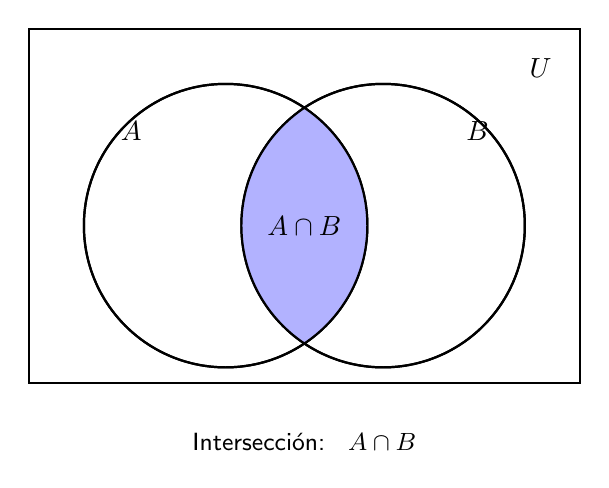
\begin{tikzpicture}[thick]
    % ─── EXPLICACIÓN DE COORDENADAS ───
    % TikZ usa coordenadas (x,y). La unidad por defecto es 1 cm.
    % El rectángulo grande va de (-2.5,-2) a (4.5,2.5).

    % Dibujamos el rectángulo del conjunto universal U
    % \draw[opciones] (x1,y1) rectangle (x2,y2);
    \draw (-2.5,-2) rectangle (4.5,2.5);
    \node at (4,2) {$U$};  % etiqueta en la esquina

    % Dibujamos el círculo A con centro en (0,0) y radio 1.8
    % \draw[opciones] (centro) circle (radio);
    \draw (0,0) circle (1.8);
    \node at (-1.2,1.2) {$A$};  % etiqueta de A

    % Dibujamos el círculo B con centro en (2,0) y radio 1.8
    \draw (2,0) circle (1.8);
    \node at (3.2,1.2) {$B$};  % etiqueta de B

    % ─── SOMBREADO DE LA INTERSECCIÓN A ∩ B ───
    % La técnica: recortar (clip) con el círculo A, y luego rellenar
    % el círculo B. El clip restringe el área de dibujo a A,
    % entonces el relleno solo afecta donde A y B se superponen.
    \begin{scope}
        \clip (0,0) circle (1.8);   % recortar al círculo A
        \fill[blue!30] (2,0) circle (1.8);  % rellenar el círculo B
    \end{scope}

    % Volvemos a dibujar los bordes para que queden encima del sombreado
    \draw (0,0) circle (1.8);
    \draw (2,0) circle (1.8);

    % Etiqueta de la intersección, centrada en (1,0)
    \node at (1,0) {$A \cap B$};

    % ─── LEYENDA ───
    \node[below] at (1,-2.5) {\small \textsf{Intersección: } $A \cap B$};
\end{tikzpicture}
\end{center}

\subsection{Otros diagramas posibles}

Con TikZ se pueden dibujar:
\begin{itemize}
    \item Árboles de decisión y de derivación
    \item Autómatas finitos (con \texttt{automata} library)
    \item Grafos (con \texttt{graphs} library)
    \item Diagramas de flujo (con \texttt{shapes.geometric} y flechas)
    \item Circuitos lógicos (compuertas AND, OR, NOT)
\end{itemize}

%% ===========================================================================
%%  SECCIÓN 5: CÓDIGO C++ CON LISTINGS
%% ===========================================================================

\section{Código C++}

\subsection{Ejemplo: verificación de las leyes de De Morgan}

El siguiente programa en C++ verifica las leyes de De Morgan
para todas las combinaciones de valores booleanos.

% ENTORNO lstlisting: muestra código fuente formateado.
% El lenguaje se hereda del estilo definido en el preámbulo (cppstyle).
%
% IMPORTANTE: DENTRO de lstlisting NO se interpreta LaTeX.
% Podés escribir &, %, #, etc. sin escaparlos.
%
% Parámetros opcionales:
%   caption = título que aparece debajo del código
%   label   = etiqueta para referencias cruzadas
%   firstnumber = desde qué número empezar

\begin{lstlisting}[caption={Verificación de las leyes de De Morgan en C++},label={codigo:dcmorgan}]
#include <iostream>
using namespace std;

int main() {
    // Probamos todas las combinaciones de p y q
    cout << "p q | !(p&&q)  !p||!q  |  !(p||q)  !p&&!q" << endl;
    cout << "------------------------------------------" << endl;

    for (int i = 0; i < 4; i++) {
        bool p = (i / 2) % 2;  // bits: 00, 01, 10, 11
        bool q = i % 2;

        bool dm1_expr = !(p && q);
        bool dm1_equiv = !p || !q;
        bool dm2_expr = !(p || q);
        bool dm2_equiv = !p && !q;

        cout << (p ? "V" : "F") << " "
             << (q ? "V" : "F") << " |   "
             << (dm1_expr ? "V" : "F") << "      "
             << (dm1_equiv ? "V" : "F") << "    |    "
             << (dm2_expr ? "V" : "F") << "      "
             << (dm2_equiv ? "V" : "F") << endl;
    }
    return 0;
}
\end{lstlisting}

\begin{observacion}
Para compilar y ejecutar este código:

\texttt{g++ -o demorgan demorgan.cpp \&\& ./demorgan}

La salida debería mostrar que las columnas de cada ley coinciden
(\texttt{!(p\&\&q)} es igual a \texttt{!p||!q}, y \texttt{!(p||q)} es igual a \texttt{!p\&\&!q}).
\end{observacion}

\subsection{Incluir código desde un archivo externo}

Si tenés un archivo \texttt{ejemplo.cpp} separado, lo podés incluir con:

% \lstinputlisting es como \includegraphics pero para código fuente.
% Usarlo es más limpio que copiar el código en el .tex.
\[
\textbackslash\texttt{lstinputlisting[style=cppstyle, caption=Mi programa]\{ejemplo.cpp\}}
\]

(sin el $\backslash$ inicial, obviamente; lo escapamos para que se vea aquí).

%% ===========================================================================
%%  SECCIÓN 6: REFERENCIA RÁPIDA
%% ===========================================================================

\section{Referencia rápida de LaTeX}

\subsection{Comandos útiles}

\begin{center}
\begin{tabular}{ll}
\toprule
\textbf{Comando} & \textbf{Qué hace} \\
\midrule
\texttt{\textbackslash{}textbf\{texto\}} & \textbf{negrita} \\
\texttt{\textbackslash{}textit\{texto\}} & \textit{cursiva} \\
\texttt{\textbackslash{}underline\{texto\}} & \underline{subrayado} \\
\texttt{\textbackslash{}texttt\{texto\}} & \texttt{monoespaciado} \\
\texttt{\textbackslash{}emph\{texto\}} & \emph{énfasis} (depende del contexto) \\
\texttt{\textbackslash{}textsc\{Texto\}} & \textsc{Versalitas} \\
\texttt{\textbackslash{}footnote\{nota\}} & pone una nota al pie\footnote{como esta} \\
\texttt{\textbackslash{}newpage} & salta a una página nueva \\
\bottomrule
\end{tabular}
\end{center}

\subsection{Caracteres especiales}

En LaTeX, estos caracteres tienen significado especial y deben escaparse:

\begin{center}
\begin{tabular}{lll}
\toprule
\textbf{Carácter} & \textbf{Comando} & \textbf{Uso} \\
\midrule
\texttt{\#} & \texttt{\textbackslash{}\#} & macro (definir comandos) \\
\texttt{\$} & \texttt{\textbackslash{}\$} & modo matemático \\
\texttt{\%} & \texttt{\textbackslash{}\%} & comentarios \\
\texttt{\&} & \texttt{\textbackslash{}\&} & alineación en tablas \\
\texttt{\_} & \texttt{\textbackslash{}\_} & subíndice \\
\texttt{\{} & \texttt{\textbackslash{}\{} & agrupar \\
\texttt{\}} & \texttt{\textbackslash{}\}} & cerrar grupo \\
\texttt{\textasciitilde} & \texttt{\textbackslash{}textasciitilde\{\}} & espacio irrompible \\
\texttt{\textasciicircum} & \texttt{\textbackslash{}textasciicircum\{\}} & superíndice \\
\texttt{\textbackslash} & \texttt{\textbackslash{}textbackslash\{\}} & inicio de comandos \\
\bottomrule
\end{tabular}
\end{center}

\subsection{Compilar el documento}

Para generar el PDF:
\begin{enumerate}
    \item Abrir una terminal en la carpeta del archivo \texttt{.tex}
    \item Ejecutar: \texttt{pdflatex template-apunte.tex}
    \item Volver a ejecutar: \texttt{pdflatex template-apunte.tex}
          (segunda pasada para resolver referencias, índice, etc.)
    \item Si usás bibliografía con BibTeX: \texttt{bibtex archivo \&\& pdflatex archivo \&\& pdflatex archivo}
\end{enumerate}

%% ===========================================================================
%%  BIBLIOGRAFÍA
%% ===========================================================================
% thebibliography: lista de referencias bibliográficas.
% El argumento {9} indica el ancho máximo de la etiqueta (para 99 referencias
% alcanza con {99}). Cada entrada es \bibitem{etiqueta} texto de la referencia.
%
% Para citar en el texto: \cite{etiqueta} (ej: \cite{Johnsonbaugh}).

\begin{thebibliography}{9}

\bibitem{Johnsonbaugh}
Richard Johnsonbaugh.
\textit{Matemáticas discretas}.
6ª edición, Pearson Educación, 2005.

\bibitem{Rosen}
Kenneth H. Rosen.
\textit{Discrete Mathematics and Its Applications}.
8ª edición, McGraw-Hill, 2019.

\bibitem{UNLP}
Cátedra de MPI I (UNLP).
\textit{Apunte de Lógica Proposicional y Conjuntos}.
Material de estudio, 2020.

\bibitem{lamport}
Leslie Lamport.
\textit{LaTeX: A Document Preparation System}.
2ª edición, Addison-Wesley, 1994.

\bibitem{wikibooks}
Wikibooks.
\textit{LaTeX}. \\
\url{https://en.wikibooks.org/wiki/LaTeX}

\end{thebibliography}

% ────────────────────────────────────────────────────────────────────────────
%  FIN DEL DOCUMENTO
% ────────────────────────────────────────────────────────────────────────────
% Todo lo que esté después de \end{document} es ignorado por LaTeX.
% Es útil para guardar notas, fragmentos de prueba, o código descartado.

\end{document}
